\pagebreak
\section{s\_simu Changes}
The \verb|s_simu| script used to run non-linear simulations from PST 3 was relatively long and objectively messy.
Work has been done to clean up the pre-existing code and functionalize sections for easier readability and process understanding.
Additionally, `stand alone mode' and 'batch mode' capabilities have been condensed into one file.
The difference between batch and stand alone mode is that the later will prompt the user for input of a system file and other simulation parameters while batch mode assumes the file to run is the \verb|DataFile.m| in the root PST directory.
\begin{itemize}
\item To use stand alone mode:\\
Run \verb|s_simu| after issuing the \verb|clear all; close all| commands.
\item To use batch mode:\\
Ensure at least 1 non-global variable is in the workspace prior to running \verb|s_simu|.
\end{itemize}


%==============================================================================
\subsection{Functionalization}
The use of a single global allowed for easier functionalization of code.
Below are some of the functions that were created from code originally found in \verb|s_simu|.

%------------------------------------------------------------------------------
\subsubsection{cleanZeros}  
The \verb|cleanZeros| function cleans all entirely zero variables from the global \verb|g| and places the names of cleared variables into the \verb|clearedVars| cell that is stored in \verb|g.sys|.
The function is executed near the end of \verb|s_simu|.

%------------------------------------------------------------------------------
\subsubsection{correctorIntegration}  
As shown in the code except below, the \verb|correctorIntegration| function performs the corrector integration step of the simulation loop to calculate the next accepted value of integrated states.
The executed code was taken directly from \verb|s_simu| and modified to work with the new global \verb|g|.

\begin{minted}[
		frame=lines,
		framesep=2mm,
		baselinestretch=1.2,
		bgcolor=gray!13,
		fontsize=\footnotesize,
	%	linenos,
		breaklines
				]{MATLAB}
function correctorIntegration(k, j, h_sol)
% CORRECTORINTEGRATION Performs x(j) = x(k) + h_sol*(dx(j) + dx(k))/2
%
%   Input:
%   k - data index for 'n'
%   j - data index for 'n+1'
%   h_sol - time between k and j
\end{minted}

It should be noted that the two integration functions write new states to the same \verb|j| data index.
Additionally, the \verb|h_sol| value is updated in \verb|i_simu| (called during the network solution) from the index of \verb|ks| referencing an \verb|h| array containing time step lengths$\ldots$\ 
While this process seemed unnecessarily confusing and sort of  round-about, it has not been changed as of this writing.

%------------------------------------------------------------------------------
\subsubsection{dcSolution}  
The portion of \verb|s_simu| that integrates DC values at 10 times the rate of the normal time step was moved into the \verb|dcSolution| function.
This has not been tested with VTS, but was functionalized to enable future development.
It appears to work as normal when using Huen's method (FTS), but a thorough testing has yet to be performed as of this writing.

Realistically, it doesn't make much sense to include a multi-rate integration routine into a variable step routine.
If DC is to be integrated into VTS, the models should be handled as all other models.
While this may defeat the purpose of VTS simulation due to DC models traditionally having very fast time constants, it is an avenue to explore should future development be desired.

%------------------------------------------------------------------------------
\subsubsection{dynamicSolution}  
As the name implies, the \verb|dynamicSolution| function performs the dynamic model calculations at data index \verb|k| by calling each required model with the input flag set to 2.
This functionalized code is again taken directly from \verb|s_simu|.

%------------------------------------------------------------------------------

\subsubsection{huensMethod}  
The default integration method used by PST is Huen's Method.
The routine has been collected into the \verb|huensMethod| function from previously existing code in \verb|s_simu|.
Mathematically speaking, Huen's method is an improved Euler method that could also be described as a two-stage Runge-Kutta method, or as a predictor-corrector method.

The description of a generalized Huen's method is as follows:
Suppose the initial conditions of an ODE $f(x,y)$ are given as $x_i$ and $y_i$.
To calculate $y_{i+1}$ using Huen's method, the derivative at $x_i$, $\dot{x_i}$, is calculated from the initial conditions.
\begin{equation}{\label{eq: huens1} }
\dot{x}_i = f(x_i, y_i)
\end{equation}\eqcaption{Huen's Method 1/4} 
\noindent A predicted point is calculated using a Forward Euler method where $h$ is the time step size.
\begin{equation}{\label{eq: huens2} }
y_p = y_i + h \dot{x}_i
\end{equation}\eqcaption{Huen's Method 2/4} 
\noindent The derivative at the predicted point is also calculated.
\begin{equation}{\label{eq: huens3} }
\dot{x}_p = f(x_{i+1}, y_p)
\end{equation}\eqcaption{Huen's Method 3/4} 
\noindent The next value for $y$, $y_{i+1}$, is calculated using an average of the two derivatives
\begin{equation}{\label{eq: huens4} }
y_{i+1} = y_i + \frac{h}{2}( \dot{x}_i + \dot{x}_p ).
\end{equation}\eqcaption{Huen's Method 4/4} 

%Essentially, 
%Huen's method uses a Forward Euler to create a prediction of the next point $y_p$ at $x_{i+1}$ using $\dot{x}_i$, 
%calculates the slope (derivative) at the predicted point to get $\dot{x}_p$, 
%then uses an average of the two derivatives $1/2(\dot{x}_t + \dot{x}_p)$
%to calculate the corrected $y_{i+1}$ at $x_{i+1}$.

As a power system solution is not just a set of differential equations, but a system of algebraic and differential equations,
\verb|huensMethod| performs the network, dynamic, DC, and monitor solutions required for each step of the method.
A block diagram of these actions is shown in Figure \ref{fig: huens block diagram}.

\begin{figure}[H]
	\centering
	\footnotesize
	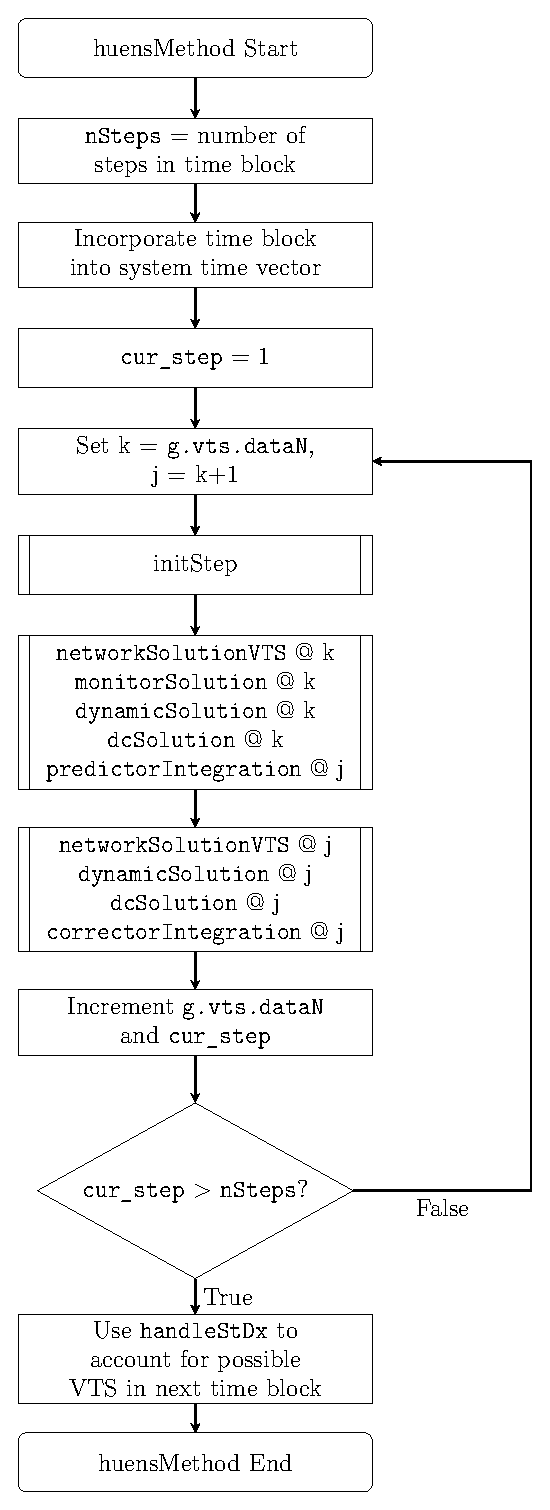
\includegraphics[height=.85\textheight]{../../one-offs/200913-huensMethodBlockDiagram/200913-huensMethodBlockDiagram}
	\caption{Huen's Method Block Diagram.}
	\label{fig: huens block diagram}
\end{figure}\vspace{-1 em}

An added benefit of functionalizing Huen's method, is that it provides a clear location to insert alternative integration routines and can act as an example as to how to accomplish such a task.

%------------------------------------------------------------------------------
\subsubsection{initNLsim}  
The \verb|initNLsim| function is a collection of code from \verb|s_simu| that performs initialization operations before a non-linear simulation.
This is essentially the creation of the various Y-matrices used for fault conditions and the calling of the dynamic models with the input flag set to 0.

%------------------------------------------------------------------------------
\subsubsection{initStep}  
Code from \verb|s_simu| that was performed at the beginning of each solution step was collected into \verb|initStep|.
Operations are related to setting values for the next step equal to current values for mechanical powers and DC currents, as well as handling machine trip flags.

%------------------------------------------------------------------------------
\subsubsection{initTblocks}  
The \verb|initiTblocks| function analyzes the global \verb|sw_con| and \verb|solver_con| to create appropriate \emph{time blocks} that are used in non-linear simulation.
Any fixed time vectors associated with time blocks that use Huen's method are also created.
Care was taken to ensure a unique time vector (no duplicate time points).
With the option to switch between fixed step and variable step  methods, this method may require slight modifications/refinements in the future.

%------------------------------------------------------------------------------
\subsubsection{initZeros}  
A large amount of code ($\approx$400 lines) in PST 3's \verb|s_simu| was dedicated to initializing zeros for data to be written to during non-linear simulation.
This code has been collected into the \verb|initZeros| function with inputs defining the desired length of vectors for normally logged data and DC data.

\begin{minted}[
		frame=lines,
		framesep=2mm,
		baselinestretch=1.2,
		bgcolor=gray!13,
		fontsize=\footnotesize,
	%	linenos,
		breaklines
				]{MATLAB}
function initZeros(k, kdc)
% INITZEROS Creates zero arrays for logged values based on passed in input
%
%   Input:
%   k - total number of time steps in the simulation
%   kdc - total number of DC time steps in the simulation
\end{minted}

%------------------------------------------------------------------------------
\subsubsection{monitorSolution}  
The \verb|monitorSolution| function takes a single input that defines the data index used to calculate any user defined line monitoring values, average system and/or area frequencies, and other interchange values for defined areas.
It should be noted that these calculations are mostly based on complex voltages that are calculated during the network solution.

%------------------------------------------------------------------------------
\subsubsection{networkSolution \& networkSolutionVTS}  
The \verb|networkSolution| function is a collection of code from \verb|s_simu| dealing with calls to dynamic models with the flag set to $1$ and Y-matrix switching.
The call to \verb|i_simu| (which updates \verb|g.k.h_sol|) is also located in this function.

The \verb|networkSolutionVTS| function is essentially the same as the \verb|networkSolution| function, except instead of relying on index number to switch Y-matricies, the switching is done based on passed in simulation time.
This was a required change when using VTS as the previous method relied on a known number of steps between switching events, and that is no longer a reality with the experimental VTS methods.

The default behavior of PST 4 is to use \verb|newtowrkSolutionVTS| which requires the input of the current data index \verb|k| and the simulation time.

%------------------------------------------------------------------------------
\subsubsection{predictorIntegration}  
The \verb|predictorIntegration| function performs the predictor (forward Euler) integration step of the simulation loop.
The code was taken directly from \verb|s_simu| and uses the same variable names adapted for use with the global \verb|g|.

\begin{minted}[
		frame=lines,
		framesep=2mm,
		baselinestretch=1.2,
		bgcolor=gray!13,
		fontsize=\footnotesize,
	%	linenos,
		breaklines
				]{MATLAB}
function predictorIntegration(k, j, h_sol)
% PREDICTORINTEGRATION Performs  x(j) = x(k) + h_sol*dx(k)
%
%   Input:
%   k - data index for 'n'
%   j - data index for 'n+1'
%   h_sol - time between k and j
\end{minted}

%------------------------------------------------------------------------------
\subsubsection{standAlonePlot}  
The \verb|standAlonePlot| function is the updated plotting routine based on user input previously found at the end \verb|s_simu|.
After a completed simulation, it is called from \verb|s_simu| if stand alone mode is detected.
Alternatively, it can be run independently from the simulation to analyze a pre-existing global \verb|g| by being invoked as \verb|standAlonePlot(1)|.

%------------------------------------------------------------------------------
\subsubsection{trimLogs}  
As there is no way to accurately predict the amount of (length of) data to be logged during a variable time step simulation, extra space is allocated, and then all logged values are trimmed to the proper length post simulation.
It should be noted that the current size allocation was arbitrary and can be altered as deemed fitting.
Typically, an extended term simulation using VTS will requires fewer steps than a fixed step method, but that is not always the case.
It's important to note that if not enough space is allocated, the simulation will crash when the code attempts to access data indices outside of the allocated range.

The \verb|trimLogs| function trims all logged values in the global \verb|g| to a given length \verb|k|.
It is executed near the end of \verb|s_simu| before \verb|cleanZeros|.

\begin{minted}[
		frame=lines,
		framesep=2mm,
		baselinestretch=1.2,
		bgcolor=gray!13,
		fontsize=\footnotesize,
	%	linenos,
		breaklines
				]{MATLAB}
function trimLogs(k)
% TRIMLOGS trims logged data to input index k.
%
%   NOTES: nCell not made via logicals - may lead to errors if fields not initialized (i.e. model not used). Issue not encountered yet, but seems possible
%
%   Input:
%   k - data index
\end{minted} 
